    \documentclass[a4paper,1cm]{article}
\usepackage{a4wide}
\usepackage[british,UKenglish,USenglish,american]{babel}
\usepackage{graphicx}
\usepackage{hyperref}
\usepackage{float}
\usepackage{siunitx}
\usepackage{rotating}
\usepackage{comment}
\usepackage{url}
\usepackage{tikz}
\newcommand{\HRule}{\rule{\linewidth}{0.5mm}}
%\numberwithin{equation}{section}
\parindent=0pt
\usepackage{float}	
\usepackage{graphicx}
\usepackage{url}
\usepackage{fullpage}
\usepackage{microtype}
\usepackage[title,titletoc]{appendix}
\usepackage[utf8]{inputenc}
\usepackage[parfill]{parskip}
\usepackage[para,online]{threeparttable}
\usepackage{booktabs}
\usepackage{listings}
\usepackage{lscape}
\usepackage{color} %red, green, blue, yellow, cyan, magenta, black, white
\definecolor{mygreen}{RGB}{28,172,0} % color values Red, Green, Blue
\definecolor{mylilas}{RGB}{170,55,241}
\usepackage[justification=centering]{caption}
\usepackage{textcomp,gensymb}
\usepackage{amsmath}
\usepackage{mathtools}
\usepackage{amsfonts}
\usepackage[gen]{eurosym}
\usepackage{color,soul}
\usepackage{pdfpages}
\usepackage{rotating,caption}
\usepackage{graphicx}
\usepackage{url}
\usepackage{mhchem}
\usepackage{fullpage}
\usepackage{microtype}
\usepackage{textgreek}
\usepackage{caption}
\usepackage{subcaption}
\usepackage{tensor}
\usepackage{todonotes}
\usepackage{ amssymb }
\usepackage{lipsum}
\usepackage[export]{adjustbox}[2011/08/13]
\setcounter{tocdepth}{2}
\textheight = 650pt
\textwidth  = 450pt
\footskip = 50pt

\definecolor{dkgreen}{rgb}{0,0.6,0}
\definecolor{gray}{rgb}{0.5,0.5,0.5}
\definecolor{mauve}{rgb}{0.58,0,0.82}

\usepackage{listings}
\lstset{
    language=Matlab,
    basicstyle=\color{black}\ttfamily\footnotesize,
    numbers=left,
    numberstyle=\tiny\color{gray},    
    stepnumber=1,                 
    numbersep=5pt,               
    commentstyle=\color{dkgreen}\itshape\ttfamily,
    keywordstyle=\color{black}\ttfamily\footnotesize,
    showstringspaces=false,
    frame=single,
    backgroundcolor=\color{white},
    keywordstyle=\color{blue}
}


\numberwithin{equation}{section}
\numberwithin{figure}{section}
\numberwithin{table}{section}
\title{Report Name}
\begin{document}
\begin{titlepage}
\begin{center} 



\includegraphics[width=6cm]{TUelogo.png}\\


\vspace*{2cm}
%titel
\HRule \\[0.4cm] { \Large \bfseries 4CM20 – Hybrid systems and control}\\[0.3cm] \HRule \\[1.5cm]

\vspace*{1cm}

\begin{center}
{\huge Takehome 2}\\
\vspace*{1cm}

\end{center}

\vspace*{2cm}

%auteurs en begeleiders
\begin{minipage}{\textwidth}\large
\begin{center}
\begin{tabular}{l r}
    
    Tim ter Huurne & 0995282\\
\end{tabular}
\end{center}
\vspace{5mm}
\begin{center}
\vspace{5mm}
Course coordinator: Prof. dr. W.P.M.H. Heemels\\
\end{center}
\end{minipage}

\vfill
%\docdate \\
\large
Eindhoven, \today\\
\end{center}
\end{titlepage}
\endcenter
\hyphenpenalty=100000
\newpage

\tableofcontents


\newpage

\section{Observer design and output-based controller design for switched systems}

In this exercise the following discrete-time switched linear system (SLS) is considered:
\begin{align}
    x_{k+1} &= A_{\sigma_k}x_k + B_{\sigma_k}u_k, \label{eq:ex1_systemx}\\
    y_k &= C_{\sigma_k}x_k.\label{eq:ex1_systemy}
\end{align}
Here $\sigma_k$ represents the active mode with $\sigma_k \in \{1,2\}$, continuous state variable $x_k \in \mathbb{R}^2$ and measurement output $y_k \in \mathbb{R}$ for discrete $k \in \mathbb{N}$. The matrices $A_1$, $A_2$, $B_1$, $B_2$, $C_1$ and $C_2$ are given by:
\begin{equation}
    A_1 = \begin{bmatrix} 0.5 & 0.5 \\ -0.5 & 1.5 \end{bmatrix}; \;
    A_2 = \begin{bmatrix} -0.5 & 0 \\ -0 & 1.5 \end{bmatrix}; \;
    B_1 = \begin{bmatrix} 0 \\ 2 \end{bmatrix}; \;
    B_2 = \begin{bmatrix} 0 \\ -4 \end{bmatrix}; \; 
    C_1 = C_2 = \begin{bmatrix} 0 & 1 \end{bmatrix}.
    \label{eq:ex1_matrices}
\end{equation}

\subsection{Exercise 1a}

In this exercise it is the objective to design an observer
\begin{equation}
    \hat{x}_{k+1} = A_{\sigma_k} \hat{x}_k + B_{\sigma_k}u_k + L_{\sigma_k} (y_k - \hat{y}_k)
    \label{eq:ex1a_observer}
\end{equation}
that asymptotically recovers the state of the system in equation \eqref{eq:ex1_systemx} - \eqref{eq:ex1_systemy}. To this end, the error is introduced as $e_k= x_k - \hat{x}_k$, by substitution of equation \eqref{eq:ex1_systemx}, \eqref{eq:ex1_systemy}, \eqref{eq:ex1a_observer} and simplification, the discrete observer error dynamics can be obtained as
\begin{equation}
    e_{k+1} = (A_{\sigma_k} - L_{\sigma_k} C_{\sigma_k}) e_k.
    \label{eq:ex1a_errordynamics}
\end{equation}
To design the observer to be asymptotically recovering the state of the system, a common Lyapunov function should be fined as
\begin{equation}
    V(e_k) = e_k^T P e_k.
    \label{eq:ex1a_CQLF}
\end{equation}
This CQLF should be strictly positive and therefore, since the error $e_k$ appears quadratically, $P$ should be positive definite. Since the Lyapunov function should be decreasing, for discrete time systems this means that $V_{k+1} - V_k > 0$, resulting in
\begin{equation}
    V_{k+1} - V_k = e_k^T (A_i - L_i C_i)^T P (A_i - L_i C_i)e_k - e_k^T P e_k < 0.
    \label{eq:ex1a_ineq}
\end{equation}
Here $i \in \sigma_t \in \{1,2\}$. To design such a Lyapunov function LMI's should be used. This can be done using the Schur complement of equation \eqref{eq:ex1a_ineq} after removing the quadratic state $e_k$ from it. This leads to the matrix inequality
\begin{equation}
    \begin{bmatrix} P & (A_i - L_i C_i)^T \\ A_i - L_i C_i P^{-1} \end{bmatrix} > 0.
\end{equation}
Note that this matrix depends on both $P$ and $P^{-1}$, which is highly non-linear. To solve this, the matrix should be pre- and post-multiplied with the same matrix, in that way the inequality still holds. This is done as
\begin{equation}
    \begin{bmatrix} I & 0 \\ 0 & P \end{bmatrix} 
    \begin{bmatrix} P & (A_i - L_i C_i)^T \\ A_i - L_i C_i P^{-1} \end{bmatrix}
    \begin{bmatrix} I & 0 \\ 0 & P \end{bmatrix} > 0.
\end{equation}
Which leads to the matrix inequality
\begin{equation}
    \begin{bmatrix} P & A_i^T P - C_i^T L_i^T P \\ PA_i - PL_i C_i & P \end{bmatrix}.
    \label{eq:ex1a_ineq2}
\end{equation}
We have to get rid of the product of $P$ and $L_i$ to make it linear, this is done with a change of coordinates $Z_i = P L_i$, this in combination with the condition that $P>0$ results in the following LMI's:
\begin{equation}
\begin{bmatrix} P & A_i^T - C_i Z_i^T \\ PA_i - Z_i C_i & P \end{bmatrix} >0 \; \; \; \text{and} \; \; \; P > 0 \; \; \forall \; i \in \{1,2\}
    \label{eq:ex1a_LMIs}
\end{equation}
This was solved with an LMI solver in Matlab and by inverting the coordinate transformation $L_i$ and $P$ are obtained as:
\begin{equation}
    L_1 = \begin{bmatrix} 0.4700 \\ 1.5326 \end{bmatrix}; \; \; 
    L_2 = \begin{bmatrix} 0.0303 \\ 1.5005 \end{bmatrix}; \; \;
    P = \begin{bmatrix} 10.7762 & 0.7870 \\ 0.7870 & 10.6421 \end{bmatrix} 
    \label{eq:ex1a_results}
\end{equation}
It can be seen that $P$ is symmetric ($P = P^T$). To validate whether these results comply with the inequalities $P>0$ and equation \eqref{eq:ex1a_ineq}. This can be done by assessing the eigenvalues of P
\begin{equation}
    \lambda_1(P) = 9.9193 \; \lambda_2(P) = 11.4990 
\end{equation}
which are all positive, meaning that $P$ is indeed positive definite. The other inequality in equation \eqref{eq:ex1a_ineq} also hold after verification. Lastly, the eigenvalues of the dynamics ($A_i - L_i C_i$) in equation \eqref{eq:ex1a_errordynamics} were checked:
\begin{equation}
    \text{for i = 1:}\; \;  \lambda_1 = 0.4702, \; \lambda_2 = -0.0028 \; \; \text{and for i = 2:}\; \; \lambda_1 = -0.5000, \; \lambda_2 = -0.0005.
\end{equation}
All these eigenvalues are smaller than 1, which means that the error will converge to zero.

\subsection{Exercise 1b}
For now we assume that the state $x_k$ of the SLS is measured completely. With this assumption, we want to design a controller $u_k = K_{\sigma_k} x_k$ such that it makes the system
\begin{equation}
    x_{k+1} = (A_{\sigma_k} + B_{\sigma_k} K_{\sigma_k}) x_k, \; \; \sigma_k \in \{1,2\}
    \label{eq:ex1b_system}
\end{equation}
globally asymptotically stable (GAS) under arbitrary switching. To this end, a mode-dependent quadratic Lyapunov function of the form 
\begin{equation}
    V(x_k, \sigma_k) = x_k^T P_{\sigma_k} x_k.
    \label{eq:ex1b_modelyap}
\end{equation}
The Lyapunov function should be strictly positive and symmetric, so $P = P^T > 0$. The Lyapunov should be decreasing over time and since we have arbitrary switching the change of the Lyapunov function should be smaller than zero regardless the switching, which results in the inequality
\begin{equation}
    V_j(x_{k+1}) - V_i(x_k) = x_k^T A_i P_j A_i x_k - x_k^T P_i x_k < 0, \; \; \forall \; i,j \in \{1,2\}.
    \label{eq:1b_lyapswitch}
\end{equation}
By removing the quadratic state $x_k$ in this equation, the following inequality is obtained:
\begin{equation}
    (A_i - B_i K_i)^T P_j (A_i - B_i K_i) - P_i < 0, \; \; \forall \; i,j \in \{1,2\}.
    \label{eq:1b_ineq1}
\end{equation}
From this inequality, the Schur complement should be used to write it towards an LMI:
\begin{equation}
    \begin{bmatrix} P_i & (A_i + B_i K_i)^T \\ A_i + B_i K_i & P_j^-1 \end{bmatrix} > 0
    \label{eq:ex1b_schur}
\end{equation}
Since there are both $P_i$ and $P_j^{-1}$ in there, some manipulation should be applied leading to: 
\begin{equation}
    \begin{bmatrix} P_i^{-1} & 0 \\ 0 & I \end{bmatrix} \begin{bmatrix} P_i & (A_i + B_i K_i)^T \\ A_i + B_i K_i & P_j^-1 \end{bmatrix}
    \begin{bmatrix} P_i^{-1} & 0 \\ 0 & I \end{bmatrix} > 0.
\end{equation}
By solving this, using the coordinate transformation $Y_i = K_i P_i^{-1}$ and using $P_i > 0$, the following LMI's are obtained:
\begin{equation}
    \begin{bmatrix} P_i^{-1} & P_i^{-1} A_i^T + Y_i^T B_i^T \\ A_i P_i^{-1} + B_i Y_i & P_j^{-1} \end{bmatrix} > 0, \; \; \text{and} \; \; P_i > 0 \; \; \forall \; i,j \in \{1,2\}.
    \label{eq:ex1b_LMI1}
\end{equation}
This leads to 6 LMI's after using all combinations of $i,j$. Solving this and reversing the coordinate transformation results in the following for $K_i$ and $P_i$:

\begin{equation}
    K_1 = \begin{bmatrix} 0.2353  & -0.7657 \end{bmatrix}, \; \; \text{and} \; \;  
    K_2 = \begin{bmatrix} -0.0074  & 0.3750 \end{bmatrix}
    \label{eq:ex1b_Kiresults}
\end{equation}
\begin{equation}
     P_1 = \begin{bmatrix} 0.0989 & 0.0146 \\ 0.0146 & 0.1067; \end{bmatrix} \; \; \text{and} \; \; 
    P_2 = \begin{bmatrix} 0.0979  & 0.0000\\ 0.0000 & 0.0917
    \end{bmatrix} 
    \label{eq:ex1b_Piresults}
\end{equation}
After checking the eigenvalues, it was confirmed that $P_i = P_i^T >0$ and the inequality in equation \eqref{eq:1b_ineq1} hold. 

\subsection{Exercise 1c}

Now a certainty equivalence controller is introduced as,
\begin{equation}
    u_k = K_{\sigma_k} \hat{x_k} = K_{\sigma_k}x_k - K_{\sigma_k} e_k.
    \label{eq:ex1c_controller}
\end{equation}

With the new state $z_k = \begin{bmatrix} x_k & e_k \end{bmatrix}^T$, the closed loop can be derived using the controller in equation \eqref{eq:ex1c_controller}. To do this, the dynamics of $x_k$ and $e_k$ need to be derived, this is done by using the observer derived in equation \eqref{eq:ex1a_observer}, the true state dynamics in equation \eqref{eq:ex1b_system} andthe error dynamics in equation \eqref{eq:ex1a_errordynamics}. By substituting the controller \eqref{eq:ex1c_controller}, the following is derived:
\begin{equation}
\begin{matrix}
    x_{k+1} =& A_{\sigma_k} x_k + B_{\sigma_k} K_{\sigma_k} x_k - B_{\sigma_k} K_{\sigma_k} e_k \\
    e_{k+1} =& A_{\sigma_k} e_k - L_{\sigma_k} C_{\sigma_k} e_k
    \end{matrix}
    \label{eq:ex1c_dynamics}
\end{equation}
By using the new state $z_k$, the following closed loop system can be written as
\begin{equation}
    z_{k+1} = M_{\sigma_k} z_k = \begin{bmatrix} A_{\sigma_k} + B_{\sigma_k} K_{\sigma_k} & -B_{\sigma_k} K_{\sigma_k} \\ O & A_{\sigma_k} - L_{\sigma_k} C_{\sigma_k} \end{bmatrix} z_k.
    \label{eq:ex1c_closedloop}
\end{equation}


\subsection{Exercise 1d}
To proof if the closed loop system in equation \eqref{eq:ex1c_closedloop} is globally asymptotically stable, a Lyapunov equation is used in the standard form:
\begin{equation}
    V (z_k) = z_k^T P_{\sigma_k} z_k
    \label{eq:ex1d_lyap}
\end{equation}
With $P_{\sigma_k} \; = \; P_{\sigma_k}^T > 0$, since the Lyapunov function should be decreasing under arbitrary switching to have GAS, the inequality
\begin{equation}
    V_j (z_{k+1}) - v_i (z_k) = z_k^T M_i^T P_j M_i z_k - z_k^T P_i z_k < 0 \; \; \forall\; \; i,j \in \{1,2\}
    \label{eq:ex1d_lyapdecreasing}
\end{equation}
should hold. To solve for $P$, this should be written as a linear matrix inequality in the following form:
\begin{equation}
    M_i^T P_j M_i - P_i < 0 \; \; \text{and} \; \; P_i > 0 \; \; \forall \; \; i,j \in \{1,2\}
\end{equation}
Solving this results in $P_1$ and $P_2$ for the Lyapunov function in equation \eqref{eq:ex1d_lyap}:
\begin{equation}
    P_1 = \begin{bmatrix}
    14.1184 & 1.8212 & 0.0430 & 0.2407 \\
    1.8212 & 9.0027 & 0.5194 & -0.2669 \\
    0.0430 & 0.5194 & 24.6995 & -3.6340 \\
    0.2407 & -0.2669 & -3.6340 & 29.4770 
    \end{bmatrix},
    \label{eq:ex1d_P1}
\end{equation}

\begin{equation}
    P_2 = \begin{bmatrix}
    13.9503 & 0.2484 & 0.0679 &  -0.4112\\
    0.2484 & 8.3545 & 0.3332 & -0.3342 \\
    0.0679 & 0.3332 & 17.1850 & -0.1528\\
    -0.4112 & -0.3342 & -0.1528 & 28.8359
    \end{bmatrix}
    \label{eq:ex1d_P2}
\end{equation}
and by looking at the eigenvalues
\begin{equation}
   \begin{matrix} eig(P_1)  =\\ \\ \\ \\ \end{matrix} \begin{matrix} 8.4039 \\ 14.6930 \\ 22.7520 \\ 31.4488 \end{matrix} \; \; \begin{matrix} \text{and}\\ \\ \\ \\ \end{matrix} \; \; 
    \begin{matrix} eig(P_2) =\\ \\ \\ \\\end{matrix}\begin{matrix} 8.3266 \\ 13.9473 \\ 17.1967 \\ 28.8551 \end{matrix}
    \label{eq:ex1d_eigP}
\end{equation}
it can be seen that $P_i = P_i^T> 0$. \cleardoublepage
\section{Computing a state-dependent and a time-dependent stabilizing switching
law for systems with shared actuation}


In this exercise two-subsystems are considered in the form
\begin{align}
    \dot{x} =& A_1 x + B_1 u_1 \label{eq:ex2_subsystemx} \\
    \dot{z} =& A_2 z + B_2 u_2. \label{eq:ex2_subsystemz}
\end{align}
Here, $x$ and $z$ the states of the first and second subsystem respectively and with
\begin{align*}
    A_1 = \begin{bmatrix}56 & -20 \\ 0 & 100 \end{bmatrix},& \; \; B_1 = \begin{bmatrix} 0 \\ 1 \end{bmatrix} \\
    A_2 = \begin{bmatrix}-21 & 10 \\ -2 & 30 \end{bmatrix},& \; \; B_2 = \begin{bmatrix} 0 \\ 1 \end{bmatrix}
\end{align*}

For these two sub-systems, there is one actuator that can only actuate on of the systems at a time. When system \eqref{eq:ex2_subsystemx} is actuated we have $u_1 = K_1 \xi$ and $u_2 = K_2 \xi$ if system \eqref{eq:ex2_subsystemz} is actuated. Here $\xi = \begin{bmatrix} x^T \\ z^T \end{bmatrix}$.

\subsection{Exercise 2a}
Since there is one actuator that can only serve one of both subsystems, these systems can be written into a switched linear system in the form
\begin{equation}
    \begin{matrix}
    \dot{\xi} = M_1 \xi \\
    \dot{\xi} = M_2 \xi
    \end{matrix}
    \label{eq:ex2a_SLS}
\end{equation}
After substitution of $u_1$ and $u_2$ in equation \ref{eq:ex2_subsystemx} and \ref{eq:ex2_subsystemz} respectively this results in
\begin{equation*}
    M_1 = \begin{bmatrix}
    A_1 & O \\ O & A_2 \end{bmatrix} + \begin{bmatrix} B_1 \\ O \end{bmatrix}K_1 \; \; \text{and} \; \: M_2 = \begin{bmatrix}
    A_1 & O \\ O & A_2 \end{bmatrix} + \begin{bmatrix} O \\ B_2 \end{bmatrix}K_1
\end{equation*}

\subsection{Exercise 2b}
The SLS introduced in equation \eqref{eq:ex2a_SLS} under periodic switching of the actuator can be considered as a hybrid automaton. With $\tau_1$ the amount of time units that the actuator is serving the first sub-system \eqref{eq:ex2_subsystemx} and $\tau_2$ the amount of time units the actuator is serving the second sub-system \eqref{eq:ex2_subsystemz}. The period of the switching thus equals to $\tau = \tau_1 + \tau_2$. A modelled hybrid automaton looks as:

\begin{figure}[H]
    \centering
    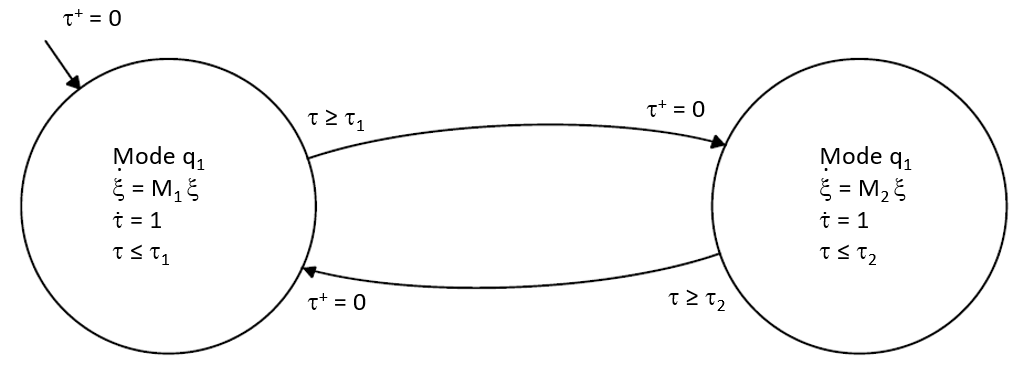
\includegraphics[width=0.8\textwidth]{Images/ex2b_hybridautomaton.PNG}
    \caption{Hybrid automaton of SLS in equation \eqref{eq:ex2a_SLS}}
    \label{fig:ex2b_hybridautomaton}
\end{figure}

\subsection{Exercise 2c}

 \cleardoublepage
\section{Reset control system}
\input{Problems/problem3}



\begin{appendices}
\input{Appendices/appendix.tex}
\end{appendices}

\clearpage

\bibliographystyle{plain}
\bibliography{BIB}

\end{document}
